% Options for packages loaded elsewhere
% Options for packages loaded elsewhere
\PassOptionsToPackage{unicode}{hyperref}
\PassOptionsToPackage{hyphens}{url}
\PassOptionsToPackage{dvipsnames,svgnames,x11names}{xcolor}
%
\documentclass[
  authoryear,
  3p]{elsarticle}
\usepackage{xcolor}
\usepackage{amsmath,amssymb}
\setcounter{secnumdepth}{5}
\usepackage{iftex}
\ifPDFTeX
  \usepackage[T1]{fontenc}
  \usepackage[utf8]{inputenc}
  \usepackage{textcomp} % provide euro and other symbols
\else % if luatex or xetex
  \usepackage{unicode-math} % this also loads fontspec
  \defaultfontfeatures{Scale=MatchLowercase}
  \defaultfontfeatures[\rmfamily]{Ligatures=TeX,Scale=1}
\fi
\usepackage{lmodern}
\ifPDFTeX\else
  % xetex/luatex font selection
\fi
% Use upquote if available, for straight quotes in verbatim environments
\IfFileExists{upquote.sty}{\usepackage{upquote}}{}
\IfFileExists{microtype.sty}{% use microtype if available
  \usepackage[]{microtype}
  \UseMicrotypeSet[protrusion]{basicmath} % disable protrusion for tt fonts
}{}
\makeatletter
\@ifundefined{KOMAClassName}{% if non-KOMA class
  \IfFileExists{parskip.sty}{%
    \usepackage{parskip}
  }{% else
    \setlength{\parindent}{0pt}
    \setlength{\parskip}{6pt plus 2pt minus 1pt}}
}{% if KOMA class
  \KOMAoptions{parskip=half}}
\makeatother
% Make \paragraph and \subparagraph free-standing
\makeatletter
\ifx\paragraph\undefined\else
  \let\oldparagraph\paragraph
  \renewcommand{\paragraph}{
    \@ifstar
      \xxxParagraphStar
      \xxxParagraphNoStar
  }
  \newcommand{\xxxParagraphStar}[1]{\oldparagraph*{#1}\mbox{}}
  \newcommand{\xxxParagraphNoStar}[1]{\oldparagraph{#1}\mbox{}}
\fi
\ifx\subparagraph\undefined\else
  \let\oldsubparagraph\subparagraph
  \renewcommand{\subparagraph}{
    \@ifstar
      \xxxSubParagraphStar
      \xxxSubParagraphNoStar
  }
  \newcommand{\xxxSubParagraphStar}[1]{\oldsubparagraph*{#1}\mbox{}}
  \newcommand{\xxxSubParagraphNoStar}[1]{\oldsubparagraph{#1}\mbox{}}
\fi
\makeatother


\usepackage{longtable,booktabs,array}
\usepackage{calc} % for calculating minipage widths
% Correct order of tables after \paragraph or \subparagraph
\usepackage{etoolbox}
\makeatletter
\patchcmd\longtable{\par}{\if@noskipsec\mbox{}\fi\par}{}{}
\makeatother
% Allow footnotes in longtable head/foot
\IfFileExists{footnotehyper.sty}{\usepackage{footnotehyper}}{\usepackage{footnote}}
\makesavenoteenv{longtable}
\usepackage{graphicx}
\makeatletter
\newsavebox\pandoc@box
\newcommand*\pandocbounded[1]{% scales image to fit in text height/width
  \sbox\pandoc@box{#1}%
  \Gscale@div\@tempa{\textheight}{\dimexpr\ht\pandoc@box+\dp\pandoc@box\relax}%
  \Gscale@div\@tempb{\linewidth}{\wd\pandoc@box}%
  \ifdim\@tempb\p@<\@tempa\p@\let\@tempa\@tempb\fi% select the smaller of both
  \ifdim\@tempa\p@<\p@\scalebox{\@tempa}{\usebox\pandoc@box}%
  \else\usebox{\pandoc@box}%
  \fi%
}
% Set default figure placement to htbp
\def\fps@figure{htbp}
\makeatother





\setlength{\emergencystretch}{3em} % prevent overfull lines

\providecommand{\tightlist}{%
  \setlength{\itemsep}{0pt}\setlength{\parskip}{0pt}}



 
\usepackage[]{natbib}
\bibliographystyle{elsarticle-harv}


\usepackage{gb4e}
\noautomath
% \usepackage[inline]{glossaries}
\usepackage{leipzig}
% \makeglossaries
\usepackage{typgloss}
\usepackage{setspace}
\usepackage{lineno}
\linenumbers
\usepackage{booktabs}
\usepackage{longtable}
\usepackage{array}
\usepackage{multirow}
\usepackage{wrapfig}
\usepackage{float}
\usepackage{colortbl}
\usepackage{pdflscape}
\usepackage{tabu}
\usepackage{threeparttable}
\usepackage{threeparttablex}
\usepackage[normalem]{ulem}
\usepackage{makecell}
\usepackage{xcolor}
\makeatletter
\@ifpackageloaded{caption}{}{\usepackage{caption}}
\AtBeginDocument{%
\ifdefined\contentsname
  \renewcommand*\contentsname{Table of contents}
\else
  \newcommand\contentsname{Table of contents}
\fi
\ifdefined\listfigurename
  \renewcommand*\listfigurename{List of Figures}
\else
  \newcommand\listfigurename{List of Figures}
\fi
\ifdefined\listtablename
  \renewcommand*\listtablename{List of Tables}
\else
  \newcommand\listtablename{List of Tables}
\fi
\ifdefined\figurename
  \renewcommand*\figurename{Figure}
\else
  \newcommand\figurename{Figure}
\fi
\ifdefined\tablename
  \renewcommand*\tablename{Table}
\else
  \newcommand\tablename{Table}
\fi
}
\@ifpackageloaded{float}{}{\usepackage{float}}
\floatstyle{ruled}
\@ifundefined{c@chapter}{\newfloat{codelisting}{h}{lop}}{\newfloat{codelisting}{h}{lop}[chapter]}
\floatname{codelisting}{Listing}
\newcommand*\listoflistings{\listof{codelisting}{List of Listings}}
\makeatother
\makeatletter
\makeatother
\makeatletter
\@ifpackageloaded{caption}{}{\usepackage{caption}}
\@ifpackageloaded{subcaption}{}{\usepackage{subcaption}}
\makeatother
\journal{Cognition}
\usepackage{bookmark}
\IfFileExists{xurl.sty}{\usepackage{xurl}}{} % add URL line breaks if available
\urlstyle{same}
\hypersetup{
  pdftitle={Sensitivity to surface-level heuristics: A case from Turkish agreement attraction},
  pdfauthor={Utku Turk},
  pdfkeywords={form-sensitivity, memory, agreement attraction},
  colorlinks=true,
  linkcolor={blue},
  filecolor={Maroon},
  citecolor={Blue},
  urlcolor={Blue},
  pdfcreator={LaTeX via pandoc}}


\setlength{\parindent}{6pt}
\begin{document}

\begin{frontmatter}
\title{Sensitivity to surface-level heuristics: A case from Turkish
agreement attraction}
\author[1]{Utku Turk%
\corref{cor1}%
}
 \ead{utkuturk@umd.edu} 

\affiliation[1]{organization={University of Maryland, College
Park, Linguistics},addressline={Marie Mount Hall},city={College
Park},postcode={20742},postcodesep={}}

\cortext[cor1]{Corresponding author}

        
\begin{abstract}
Surface level does not affect it, but within-experiment statistics
effect the findings.
\end{abstract}





\begin{keyword}
    form-sensitivity \sep memory \sep 
    agreement attraction
\end{keyword}
\end{frontmatter}
    

\section{Introduction}\label{introduction}

Sentence processing is shaped not only by grammatical constraints but
also by plausibility, frequency, task-specific factors, and phonological
processes. Recent work shows that such influences can substantially
modulate reading and judgment behavior
\citep{LauraMalsbug24, ArehalliWittenberg2021, HammerlyEtAl2019, LogacevVasishth2016}.
Form-based overlap between elements in a sentence can also influence how
sentences are processed. A substantial body of work has shown that the
parser and the production system are sensitive not only to syntactic or
semantic relations but also to the surface form of words. These effects
have been taken to suggest that, under certain circumstances, speakers
and comprehenders rely on shallow or heuristic cues to complete
dependencies. \citet{AchesonMacDonald2011}, for example, found that
participants showed slower reading times when the subjects of the two
embedded clauses share phonological similarity
(\emph{baker}-\emph{banker} in \ref{baker}
vs.~\emph{runner}-\emph{banker} in \ref{runner}). Moreover, participants
were less accurate in answering comprehension questions with
phonological overlap present. Related work in short-term memory and word
recognition shows similar effects---items that overlap phonologically or
morphologically are more confusable and more easily retrieved (Copeland
\& Radvansky, 2001; Rastle \& Davis, 2008).

\begin{exe}
\ex \label{baker} The baker that the banker sought bought the house.
\ex \label{runner} The baker that the banker sought bought the house..
\end{exe}

One domain in which these influences are observed is the research on
agreement attraction as in (\ref{og}), a phenomenon in which a verb
erroneously agrees with a nearby noun rather than its grammatical
subject, producing so-called grammaticality illusions
\citep{BockMiller:1991, PearlmutterGarnseyBock:1999}. This effect have
been robustly attested in many languages with various methodologies
{[}to name a few{]}. \citet{BockEberhard1993} tested whether attractors
that only sound plural, pseudoplurals such as \emph{course}
\ref{pseudo}, increase agreement errors compared to true plural nouns
(\ref{true-pl}). They reasoned that if participants rely on phonological
cues rather than abstract features, words ending with plural-like sounds
(/s/ or /z/) should behave like true plurals. Participants completed
sentence preambles such as (\ref{ex:bockeberhard93}), where the head
noun (\emph{player}) was singular but the attractor varied in form. They
found that pseudoplural attractors did not increase plural agreement
rates.

\begin{exe} 
\ex[*]{\label{og} The player on the courts are tired from a long-game.}
\ex \label{ex:bockeberhard93}
\begin{xlist}
    \ex \label{pseudo} {Pseudoplural Attractor} \\ The {player} on the {course} \ldots{}
    \ex \label{true-sg} {Singular Attractor} \\ The {player} on the {court} \ldots{}
    \ex \label{true-pl} {Plural Attractor} \\ The {player} on the {courts} \ldots{}
\end{xlist}
\end{exe}

Even though modulation from a pure phonological similarity was not
found, several experiments have manipulated morphological case
similarity between controllers and attractors, reasoning that syncretism
or surface ambiguity could enhance competition during retrieval or
interfere in production {[}PAPERS{]}. For example,
\citet{HartsuikerEtAl2003} used the overlap between accusative and
nominative forms of feminine determiners in German and compared these
ambiguous forms to distinctively marked dative forms. Participants
produced more agreement errors when the preambles contained two noun
phrases whose determiners were not distinctively marked, as in
(\ref{ger-amb}), compared to cases where the attractor could be
distinguished by form alone, as in (\ref{ger-dist}). Crucially, this
additive effect was limited to feminine nouns, the only gender showing
nominative--accusative syncretism in plural forms while other nouns
showed the base effect of plural.

\begin{exe}
\ex \label{ger}
\begin{xlist}
\ex \label{ger-amb}
\gll Die Stellungnahme gegen die Demonstration-en\\
the.F.NOM.SG position against the.F.ACC.PL demonstration-PL\\
\glt `The position against the demonstrations'
\ex \label{ger-dist}
\gll Die Stellungnahme zu den Demonstration-en\\
the.F.NOM.SG position on the.F.DAT.PL demonstration-PL\\
\glt `The position on the demonstrations'
\end{xlist}
\end{exe}

Similar effects of surface similarity are also found in comprehension
studies. \citet{Slioussar2018}, for example, showed that phonological
overlap affects the reading pattern and accuracy of participants in
Russian agreement. A group of accusative marked nouns in Russian
surfaces ambiguously with their nominative counterparts when they are
plural (\ref{RusAccSg}-\ref{RusAccPl}). Meanwhile, it is possible to
assign a different case to the attractors using a different preposition
as in (\ref{RusGenSg}-\ref{RusGenPl}). Crucially, in her experiment the
genitive marked plural nouns were not ambiguous with their nominative
counterparts. \citet{Slioussar2018} showed that participants not only
exhibited faster reading times at the verb in (\ref{RusAccPl}) compared
to (\ref{RusAccSg}), but also judged sentences with a plural attractor
as grammatical more often. These effects of plural attractor were only
present in cases with ambiguous case marking.

\begin{exe}
\ex
\begin{xlist}
\ex \label{RusAccSg}
\gll ssylka na sajt byli dany.\\
link[NOM.SG] to {website[ACC.SG($\neq$NOM.PL)]} were given\\
\ex \label{RusAccPl}
\gll ssylka na sayty byli dany.\\
link[NOM.SG] to {website[ACC.PL($=$NOM.PL)]} were given\\
\glt `The link to the website(s) were given.'
\ex \label{RusGenSg}
\gll material dlja kry\c{s}i byli brakovannymi.\\
material[NOM.SG] for {roof[GEN.SG($=$NOM.PL)]} were defective\\
\ex \label{RusGenPl}
\gll material dlja kry\c{s} byli brakovannymi.\\
material[NOM.SG] for {roof[GEN.PL($\neq$NOM.PL)]} were defective\\
\glt `The material for the roof(s) were defective.'
\end{xlist}
\end{exe}

However, a more intriguing aspect of the study by \citet{Slioussar2018}
is her results with respective to attractors marked with genitive
singular. Another interesting characterics of Russian is such that a
subset of \emph{singular} genitive nouns share the same form with their
plural nominal counterpart. In addition to plural nouns not increasing
grammatical judgments to ungrammatical sentences and not creating a
reading advantage, the verbs of singular attractors were read faster and
resulted in more `yes' responses to grammaticality judgments.

In this aspect, the findings of \citet{Slioussar2018} targets the
initial question raised by \citet{BockEberhard1993}: whether the pure
phonological similarity can drive the agreement attraction effects.
Given the contention of initial findings of \citet{BockEberhard1993}
with Russian data and the theoretical importance of the empirical
generalization, we tested whether we could find attraction effects with
another type morphologically rich language, Turkish. Turkish, an
almost-strict agglutinative language, presents another typological
aspects of morphological marking. English, a predominantly analytic
language that uses separate words, such as prepositions, particles, and
auxiliary verbs, to express grammatical meaning rather than relying on
inflections or affixes attached to words did not show an effect of pure
phonological overlap. Meanwhile, Russian, a fusional language in which a
single affixal morpheme can express multiple grammatical meanings,
exhibited the effect of phonological overlap. Turkish represents another
group of languages in which there is close to 1-to-1 mapping between
gramatical meanings and affixal morphemes.

In this paper, we test whether pure phonological overlap can derive
agreement attraction effects in two high-powered speeded acceptability
judgment experiments. To this end we use Turkish, a language where
verbal and nominal plural marking share the same surface form, the
suffix --lAr. We use reduced relative clause (RRC) structures, in which
the verb with the plural marking alone can appear as the attractor
(\ref{rrc-intro}). Importantly, Turkish --lAr syncretism here is not
feature-ambiguous (as in cases of syncretism); it is a form-only overlap
that does not share possible argument status with the subject. Even when
the RRC can surface without its head as the subject, they cannot control
the agreement (\ref{rrc-subject}).

\begin{exe}
\ex \label{rrc-intro}
\gll Gör-dük-ler-i çocuk koş-tu-(*lar).\\
go-NMLZ-PL-POSS kid[NOM] run-PST-(*PL)\\
\glt `The kid that (they) saw ran.'
\ex \label{rrc-subject}
\gll Gör-dük-ler-i koş-tu-(*lar).\\
go-NMLZ-PL-POSS run-PST-(*PL)\\
\glt `(The kid) that (they) saw ran.'
\end{exe}

In Experiment 1, we tested the form hypothesis directly by comparing
ungrammatical sentences with verbal-plural vs.~verbal-singular
attractors. Experiment 2 replicated this design but included additional
nominal-attractor items from a previous Turkish attraction study
\citep{TurkLogacev2024}, allowing us to test whether the distribution of
item types and the presence of genuine attraction-inducing elements
modulates the outcome. Across both experiments, we found no evidence
that verbal --lAr induces attraction, even when canonical nominal
attractors are present in the same session. This pattern aligns with
prior findings in general attraction literature and Turkish agreement
attraction, namely surface-form overlap alone does not drive agreement
illusions. Rather, attraction appears to depend on abstract feature
overlap between potential controllers and agreement probes. In this
lights, findings of \citet{Slioussar2018} becomes even more surprising
given that singular attractors that are homophonous with plurals were
able to induce attraction effects. One way to co\ldots{} these findings
is to refer to types of morphological encoding or the functional utility
of morphemes in specific languages following \citet{KeshevDillon2024}.

\subsection{Primer on Attraction Accounts and Phonological
Modulation}\label{primer-on-attraction-accounts-and-phonological-modulation}

Agreement errors in sentences like (\ref{og}) have been treated either
as a failure of feature reconcilation or a failure of memory encoding.

The former set of accounts explain these errors as a by-product of how
number feature of a phrase is calculated in real-time
\citep{BockMiller:1991, EberhardEtAl2005, HammerlyEtAl2019}. For
example, \citet{EberhardEtAl2005}, in their Marking and Morphing
account, argue that speakers and comprehenders does not necessarily
create binary singular or plural representation, instead they consider
various number related information in a phrase and create a continuous
value. This related information include (i) the inherent conceptual
number of the head of phrase, namely collectiveness or distributiveness
of a noun, (ii) grammatical number markings on all nouns within a phrase
weighted by their syntactic distance, and (iii) idiosyncretic (scissors)
or grammatical (books) presence of a plural marking. The errors
probabilistically arise when additional plurality features from
different sources contribute to the final number representation of a
phrase. Because this account ties attraction to various sources
including the presence of a plural morpheme, it could in principle
accommodate effects of surface-form similarity. However, this surface
form similarity effects should be limited to the cases where it can be
associated with a plural number marking, and should not arise with pure
phonological similarities.

On the other hand, the latter set of accounts claim that the initial
representation is not erroneous, but speakers are sometimes unable to
correctly retrieve the controller
\citep{WagersEtAl:2009, Dillon2013a, RyskinEtAl2021}. For example,
\citet{WagersEtAl:2009}, in their memory account, assumes a cue-based
retrieval model in which the verb cues a search for a memory chunk
matching relevant cues for subjecthood and number. In the ungrammatical
attraction sentences as in (\ref{og}), each of chunks for `courts' and
`player' matches a subset of relevant cues. In these partial match
scenarios, erroneously retrieval of the attractor may lead comprehenders
to judge the sentence grammatical. In this framework, surface-form
overlap affects processing only if it contributes to cue overlap. For
example, plural morphology or phonological endings could influence
retrieval if the system treats them as diagnostic of plural number.
Because the model allows cues to be weighted differently depending on
their reliability, it trivially accounts for cross-linguistic
variability in the role of case marking and other morphosyntactic
features.

The two main set of explanations, therefore, make different predictions
for the influence of surface similarity. Feature reconcilation accounts
predict form-based attraction if overlapping phonology also results in
overlapping morphological representations, whereas cue-based retrieval
predicts form effects only when they are encoded as retrieval cues,
i.e.~relevant for predictions. Indeed, \citet{LagoEtAl2019} previously
argued that Turkish genitive case marking is associated with subjecthood
in Turkish, due to they marking subjects in embedded clause, and thus
derives attraction effects in Turkish. A similar account from Dillon and
colleagues pushed for sensitivity to looking like a controller
\citep{BhatiaDillon2022, BleotuDillon2024}. However, both of these
accounts argue for distributional or within-item possibility of being a
controller, instead of surface level similarity. Turkish verbal -lAr
presents a clear dissociation between form-association with subjecthood
and being a controller. As we previously noted, they can surface as a
subject, they do look like a controller, but they cannot control the
agreement and they are not possible controllers. In this aspect, Turkish
verbal -lAr is similar to Russian genitive cases. If verbal -lAr, like
Russian genitive case, induce attraction errors, current models of
attraction need to be revised to include phonological similarity beyond
being a possible controller.

\section{Experiment 1: Testing Form-Driven
Processing}\label{experiment-1-testing-form-driven-processing}

\subsection{Participants}\label{participants}

We recruited 80 undergraduate students to participate in the experiment
in exchange for course credit. All participants were native Turkish
speakers, with an average age of 21 (range: 18 -- 31). The experiment
was carried out following the principles of the Declaration of Helsinki
and the regulations concerning research ethics at Bogazici University.
All participants provided informed consent before their participation
and their identities were completely anonymised.

\subsection{Materials}\label{materials}

We used 40 sets of sentences like (\ref{exp}), in which we manipulated
(i) the number of the attractor and (ii) the number agreement on the
verb. Both plural markings were marked with the suffix -ler/-lar, while
the singular number and singular agreement were marked by its absence.

\begin{exe}
\ex \label{exp}
\begin{xlist}
\ex[]{\label{ss}
\gll Tut-tuğ-u aşçı mutfak-ta sürekli zıpla-dı.\\
hire-NMLZ-POSS cook[NOM] kitchen-LOC non.stop jump-PST\\
\glt `The cook they hired$_{sg}$ jumped$_{sg}$ in the kitchen non-stop.'}
\ex[*]{\label{sp}
\gll Tut-tuğ-u aşçı mutfak-ta sürekli zıpla-dı-lar.\\
hire-NMLZ-POSS cook[NOM] kitchen-LOC non.stop jump-PST-PL\\
\glt `The cook they hired$_{sg}$ jumped$_{pl}$ in the kitchen non-stop.'}
\ex[]{\label{ps}
\gll Tut-tuk-lar-ı aşçı mutfak-ta sürekli zıpla-dı.\\
hire-NMLZ-PL-POSS cook[NOM] kitchen-LOC non.stop jump-PST\\
\glt `The cook they hired$_{pl}$ jumped$_{sg}$ in the kitchen non-stop.'}
\ex[*]{\label{pp}
\gll Tut-tuk-lar-ı aşçı mutfak-ta sürekli zıpla-dı-lar.\\
hire-NMLZ-PL-POSS cook[NOM] kitchen-LOC non.stop jump-PST-PL\\
\glt `The cook they hired$_{pl}$ jumped$_{pl}$ in the kitchen non-stop.'}
\end{xlist}
\end{exe}

All sentences were adapted by previous studies in Turkish agreement
attraction \citep{LagoEtAl2019, TurkLogacev2024}. Sentences started with
a complex subject NP like `tuttukları aşçı' `the cook they hired,' in
which the nominalized relative clause functioned as the attractor, and
the head noun were bare. Because the plural marking on nominals is not
optional and the head noun was singular, absent of -lar, in all
conditions, sentences with plural verb agreement were ungrammatical. To
inhibit participants from forming a task-related strategy in which they
deemed the sentence ungrammatical upon seeing a plural verb, half of our
fillers included plural grammatical verbs, while the other half included
singular ungrammatical verbs.

\subsection{Procedures}\label{procedures}

The experiment was run online, using the web-based platform Ibex Farm
\citep{Drummond2013}. Each experimental session took approximately 25
minutes to complete. Participants provided demographic information and
gave informed consent to participate in the experiment. They then
proceeded to read the instructions and were given nine practice trials
before the experiment began.

Each trial began with a blank screen for 600 ms, followed by a
word-by-word RSVP presentation of the sentence in the center of the
screen, followed by a prompt to indicate their acceptability judgment.
Sentences were presented word-by-word in the center of the screen in 30
pt font size, at a rate of 400 ms per word. Participants saw a blank
screen for 100 ms between each word, and to see the next item, they
needed to press the space key. Participants were asked to press the key
P to indicate that a sentence is acceptable and Q to indicate that the
sentence is unacceptable. They were instructed to provide judgments as
quickly as possible. During the practice, but not during the experiment,
a warning message in red font appeared if they did not respond within
5,000 ms.

Participants saw 40 experimental and 40 filler sentences. Experimental
sentences were distributed among four different lists according to a
Latin-square design. Every participant saw one version of the experiment
with a specific list and one item per condition.

\subsection{Analysis and Results}\label{analysis-and-results}

Participants showed high accuracy in both grammatical (M = 0.94, CI =
{[}0.92,0.95{]}) and ungrammatical filler sentences (M = 0.92, CI =
{[}0.9,0.93{]}), indicating that they understood the task and performed
it reliably.

Figure 1 presents the overall means and credible intervals for `yes'
responses across experimental conditions. As shown, ungrammatical
sentences with plural attractors were rated as acceptable as their
counterparts with singular attractors (M = 0.06 and 0.05, CI = {[}0.04,
0.07{]} and {[}0.03, 0.07{]} for singular and plural attractors,
respectively).

On the other hand, accuracy in grammatical conditions was modulated by
the number of the attractor in an unexpected way. Participants rated
grammatical sentences with singular attractors as grammatical less often
(M = 0.92, CI = {[}0.9,0.94{]}) compared to their counterpars with
plural attractors (M = 0.95, CI = {[}0.93,0.96{]}).

\begin{figure}[H]

{\centering \pandocbounded{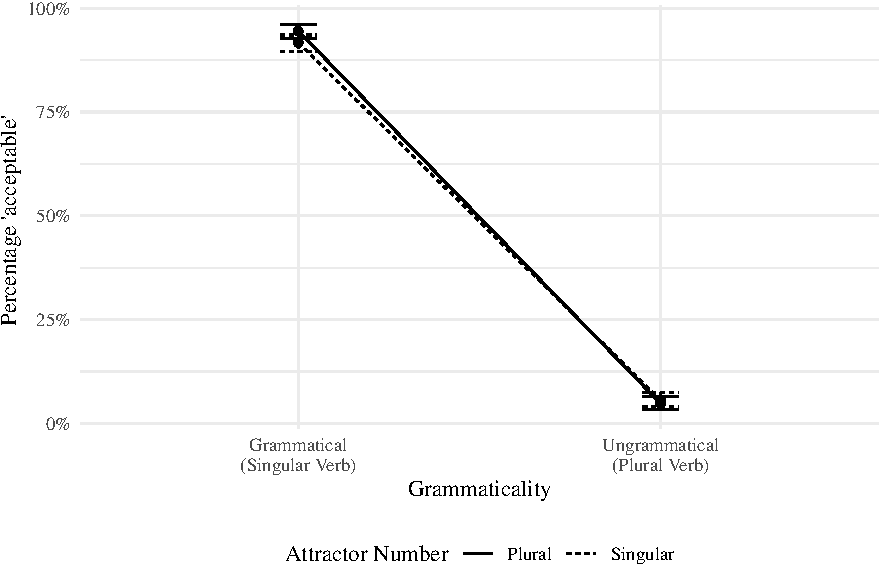
\includegraphics[keepaspectratio]{paper_files/figure-pdf/exp1-condition-means-1.pdf}}

}

\caption{Mean proportion of `acceptable' responses by grammaticality and
attractor number. Error bars show 95\% Clopper--Pearson confidence
intervals.}

\end{figure}%

These descriptive trends were confirmed by our Bayesian mixed-effects
models implemented in brms, assuming a Bernoulli logit link. The model
was fitted to the binary \emph{yes/no} responses and included fixed
effects for Grammaticality and Attractor Number and their interaction,
and random intercepts and slopes for both subjects and items.

Posterior estimates are summarized in Figure 2. The model revealed a
positive effect of grammaticality (\(\beta\) = 5.92 {[}5.41, 6.46{]},
P(\(\beta\) \textgreater{} 1.00)), but no reliable main effect of
attractor number (\(\beta\) = 0.15 {[}-0.19, 0.51{]}, P(\(\beta\)
\textgreater{} 0.81)). On the other hand, there was a small but positive
interaction (\(\beta\) = 0.66 {[}-0.02, 1.38{]}, P(\(\beta\)
\textgreater{} 0.97)). To clarify the effects' presence in grammaticals
only, we fitted two more models that is fitted to the subset of the
data. While the model fitted to grammatical conditions only showed an
effect of attractor number (\(\beta\) = 0.51 {[}0.06, 1.00{]},
P(\(\beta\) \textgreater{} 0.99)), the model fitted to ungrammatical
conditions did not provide evidence for the effect of number
manipulation (\(\beta\) = -0.05 {[}-0.45, 0.37{]}, P(\(\beta\)
\textgreater{} 0.99)). These results suggest that the presence of a
plural attractor did not increase the acceptability of ungrammatical
sentences, nor was this relationship modulated by grammaticality.

\begin{figure}[H]

{\centering \pandocbounded{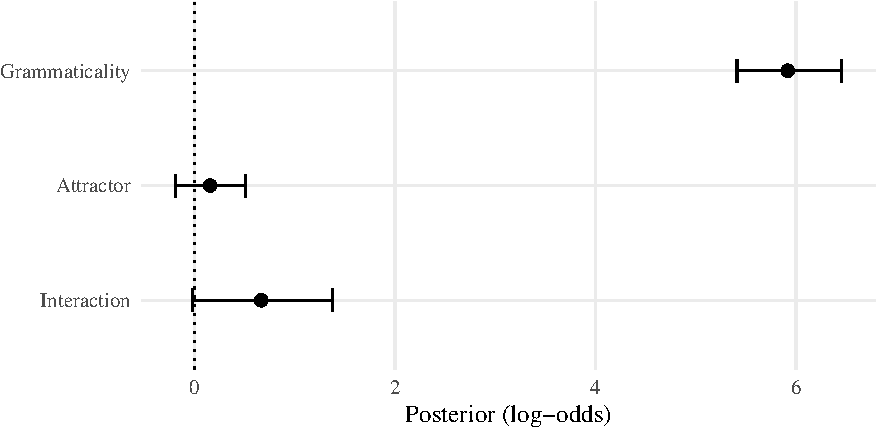
\includegraphics[keepaspectratio]{paper_files/figure-pdf/exp1-fixed-effects-1.pdf}}

}

\caption{Posterior means and 95\% credible intervals for fixed effects
in the two Bayesian models. The x-axis shows the posterior mean
(log-odds scale). The blue intervals correspond to the model in which a
positive interaction was assumed, and the orange intervals to the model
in which it was not.}

\end{figure}%

\subsection{Discussion}\label{discussion}

\begin{itemize}
\tightlist
\item
  No attraction effect
\item
  There is an unexpected effect, which is might be due to interaction
  between the plausability and the availability of a referent. While the
  plural morpheme can give a general reading, the singular RC probably
  requires an overt referent. It is outside of the scope of this paper.
\end{itemize}

However, both group of accounts generally are underspecified in terms of
how meta-linguistic information should be integrated to the
inter-sentential dependency mechanisms. Recently, a growing literature
have been testing how different types of additional sources that are
independent of the linguistic information affects these errors. Recent
experiments show that even small changes in task expectations can alter
attraction patterns. For example, \citet{LauraMalsbug24} found that
varying the practice structure and task demands (reading vs.~judgment)
affected reading times at the verb in sentences as in (\ref{malsburg}).
In a series of high-powered self-paced reading tasks, they found that
when participants answered a comprehension question after each trial,
reading times at the verb `admires' did not differ between
(\ref{malsburg-singer}) and (\ref{malsburg-singers}). However, when
participants were asked to judge grammaticality instead, they spent more
time reading the verb `admires' in (\ref{malsburg-singers}), suggesting
that processing mechanisms can change depending on the expected task.

\begin{exe}
\ex \label{malsburg}
\begin{xlist}
\ex \label{malsburg-singer} The singer that the actor openly admires apparently received broad international recognition.
\ex \label{malsburg-singers} The singers that the actor openly admires apparently received broad international recognition.
\end{xlist}
\end{exe}

A related set of findings came from \citet{HammerlyEtAl2019}. They
challenge long-standing assumption that the agreement errors only
surfaced in ungrammatical sentences such as (\ref{og}), but not in
grammatical sentences as in (\ref{og-g}). It has been repeatedly shown
that a plural noun increased participants' likelihood to erroneously
judge ungrammatical sentences as grammatical; however, participants
rarely misidentified grammatical sentences as ungrammatical even when
there is an attractor. \citet{HammerlyEtAl2019} showed that similar
effect surfaced in grammatical sentences when participants' a priori
expectations about the experiment is altered. They manipulated the
instructions and the number of ungrammatical in an experiment so that
participants expected to see more ungrammatical sentences than
grammatical sentences. With reduced bias towards grammaticality, they
found that the presence of a plural nearby noun affected how speakers
completed ungrammatical sentences (\ref{og}) and grammatical sentences
(\ref{og-g}) {[}see TURK2022 for acceptability{]}.

\begin{exe}
\ex[]{\label{og-g}The key to the cabinets is rusty.}
\end{exe}

\section{Experiment 2: Testing Within-Experiment Statistical
Sensitivity}\label{experiment-2-testing-within-experiment-statistical-sensitivity}

\subsection{Participants}\label{participants-1}

We recruited 95 undergraduate students to participate in the experiment
in exchange for course credit. All participants were native Turkish
speakers, with an average age of 21 (range: 18 -- 30). The experiment
was carried out following the principles of the Declaration of Helsinki
and the regulations concerning research ethics at Bogazici University.
All participants provided informed consent before their participation
and their identities were completely anonymised.

\subsection{Materials}\label{materials-1}

The same materials were used with Exp1. We added items from
\citet{TurkLogacev2024} as an additional condition for nominal cases.

\subsection{Procedures}\label{procedures-1}

The same procedure with Experiment 1 was used.

\subsection{Analysis and Results}\label{analysis-and-results-1}

Participants showed high accuracy in both grammatical (M = 0.95, CI =
{[}0.94,0.96{]}) and ungrammatical filler sentences (M = 0.94, CI =
{[}0.93,0.95{]}), indicating that they understood the task and performed
it reliably.

Figure 3 presents the overall means and credible intervals for `yes'
responses across experimental conditions, as well as the previous data
from \citet{TurkLogacev2024}, which is quite similar to the magnitude of
\citet{LagoEtAl2019}. As shown, in our study, participant gave more
`yes' responses to ungrammatical sentences with plural genitive-marked
nominal attractors (M = 0.12, CI = {[}0.09,0.15{]}) compared to their
singular counterparts (M = 0.12, CI = {[}0.09,0.15{]}).

However, similar increase in acceptability was not found with relative
clause attractors (M = 0.05 and 0.05, CI = {[}0.03, 0.07{]} and {[}0.03,
0.07{]} for singular and plural attractors, respectively). Participants
rated grammatical sentences similarly independent of the attractor
number or attractor type.

\begin{figure}[H]

{\centering \pandocbounded{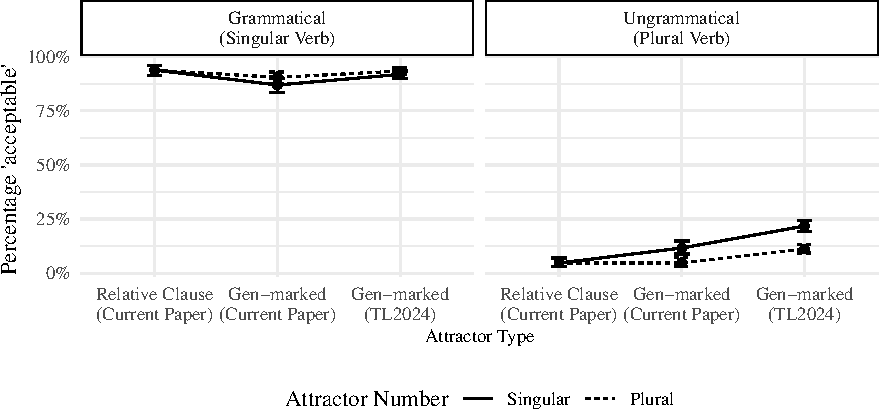
\includegraphics[keepaspectratio]{paper_files/figure-pdf/exp2-condition-means-1.pdf}}

}

\caption{Mean proportion of `acceptable' responses by grammaticality,
attractor number and attractor type. Error bars show 95\%
Clopper--Pearson confidence intervals.}

\end{figure}%

Our models also showed similar results, assuming a Bernoulli logit link.
The model was fitted to the binary \emph{yes/no} responses and included
fixed effects for Grammaticality, Attractor Number, and Attractor Type
and their interaction, along with random intercepts and slopes for both
subjects and items. Since our main question was whether
within-experiment statistics affect the grammaticality magnitudes, we
fitted another model with genitive marked nominals from data from our
experiment and \citet{TurkLogacev2024}.

Talk about the important points. not all of them. attraction effect
existed. and it also manipulated as a three way which tells us that
participant only did in a single type.

as for our second model, we present the illusion estimate as a function
of experiment. Attraction:Current, Attraction:TL24

\begin{figure}[H]

{\centering \pandocbounded{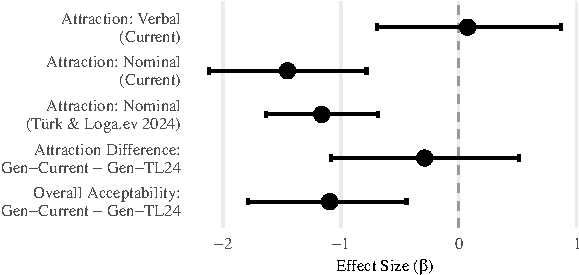
\includegraphics[keepaspectratio]{paper_files/figure-pdf/exp2-fixed-effects-1.pdf}}

}

\caption{Posterior means and 95\% credible intervals for fixed effects
in the two Bayesian models. The x-axis shows the posterior mean
(log-odds scale). The blue intervals correspond to the model in which a
positive interaction was assumed, and the orange intervals to the model
in which it was not.}

\end{figure}%

\subsection{Discussion}\label{discussion-1}

\begin{itemize}
\tightlist
\item
  Goal: test whether attraction changes when both attractor types occur
  in one experiment.
\item
  Participants: 95 Turkish speakers.
\item
  Design: 2 × 2 × 2 (Grammaticality × Attractor Number × Attractor Type
  {[}nominal vs verbal{]}).
\item
  Procedure \& analysis: same as Experiment 1.
\item
  Results:

  \begin{itemize}
  \tightlist
  \item
    Attraction replicated for nominal attractors (Δ ≈ 0.07).
  \item
    Verbal attractors again showed null effect.
  \item
    Global decline in yes-responses relative to earlier studies →
    participants became more conservative.
  \end{itemize}
\item
  Discussion:

  \begin{itemize}
  \tightlist
  \item
    Exposure to verbal conditions reduced attraction magnitude overall.
  \item
    Indicates participants adapt to statistical properties of the task.
  \item
    Aligns with learning-based cue-weighting accounts (Haskell et
    al.~2010).
  \end{itemize}
\end{itemize}

\section{General Discussion}\label{general-discussion}

\begin{itemize}
\tightlist
\item
  Synthesis:

  \begin{itemize}
  \tightlist
  \item
    No evidence for surface-form matching; effects are feature-based.
  \item
    Attraction magnitude changes with condition distribution → adaptive
    tuning.
  \end{itemize}
\item
  Interpretation:

  \begin{itemize}
  \tightlist
  \item
    Supports an adaptive parser sensitive to within-experiment
    statistics.
  \item
    Challenges ``shallow'' or ``good-enough'' accounts that attribute
    attraction to phonological overlap.
  \end{itemize}
\item
  Broader implication:

  \begin{itemize}
  \tightlist
  \item
    Agreement processing is flexible and probabilistic; illusions arise
    from learned cue validity.
  \end{itemize}
\item
  Limitations:

  \begin{itemize}
  \tightlist
  \item
    Syntactic depth asymmetry (verbal attractors more embedded).
  \item
    Need future designs equating structure (e.g., embedded-object
    attractors).
  \end{itemize}
\item
  Conclusion:

  \begin{itemize}
  \tightlist
  \item
    Turkish attraction effects arise from abstract feature retrieval not
    surface level shallow form-matching.
  \item
    The evaluation of abstract features are modulated by distributional
    learning within the experiment.
  \end{itemize}
\end{itemize}

\section*{References}\label{references}
\addcontentsline{toc}{section}{References}

\newcommand{\doi}[1]{\href{http://dx.doi.org/#1}{http://dx.doi.org/#1}}
\begingroup
\raggedright
\singlespacing

\renewcommand{\bibsection}{}
\bibliography{bibliography.bib}

\endgroup





\end{document}
